\section{Conclusion}

<<<<<<< .mine
In this work, we resented a novel technique to align segmentation
hierarchies. We proposed a method to learn and predict the scale of
segments. We then formulated the scale prediction for the segments in
a hierarchy as a graph label problem, which is solved by dynamic
programming. With the labeled scales as constraints, we then re-align
the segmentation hierarchies by streching the UCM maps.  The method
were evaluted on four different segmentation hierarchies, and it
consistently improve the quality of the hierarchies.  We also showed
that the improvement of segmentation hierarchies by our alignment is
reflected well to a high-level task of proposing object masks.
=======
In this work, we have presented a novel technique to align segmentation tree. First we predict the scales of regions by mid-level features. We formulated the problem of finding anchor slice as a scale labelling problem, which can solved efficiently by dynamic programming. The final output is done by linear interpolation using the anchor slice. The results on BSDS500 dataset indicate that our algorithm significantly and consistently improves hierarchical segmentation. Our approach provides better alignment for depth and scale, both within a image and across images. Furthermore, we prove that alignment can improve object segmentation, thus high-level vision tasks can in principle benefit from our approach.
>>>>>>> .r54

<<<<<<< .mine
=======
\begin{figure*}
\begin{center}
\begin{tabular}{c}
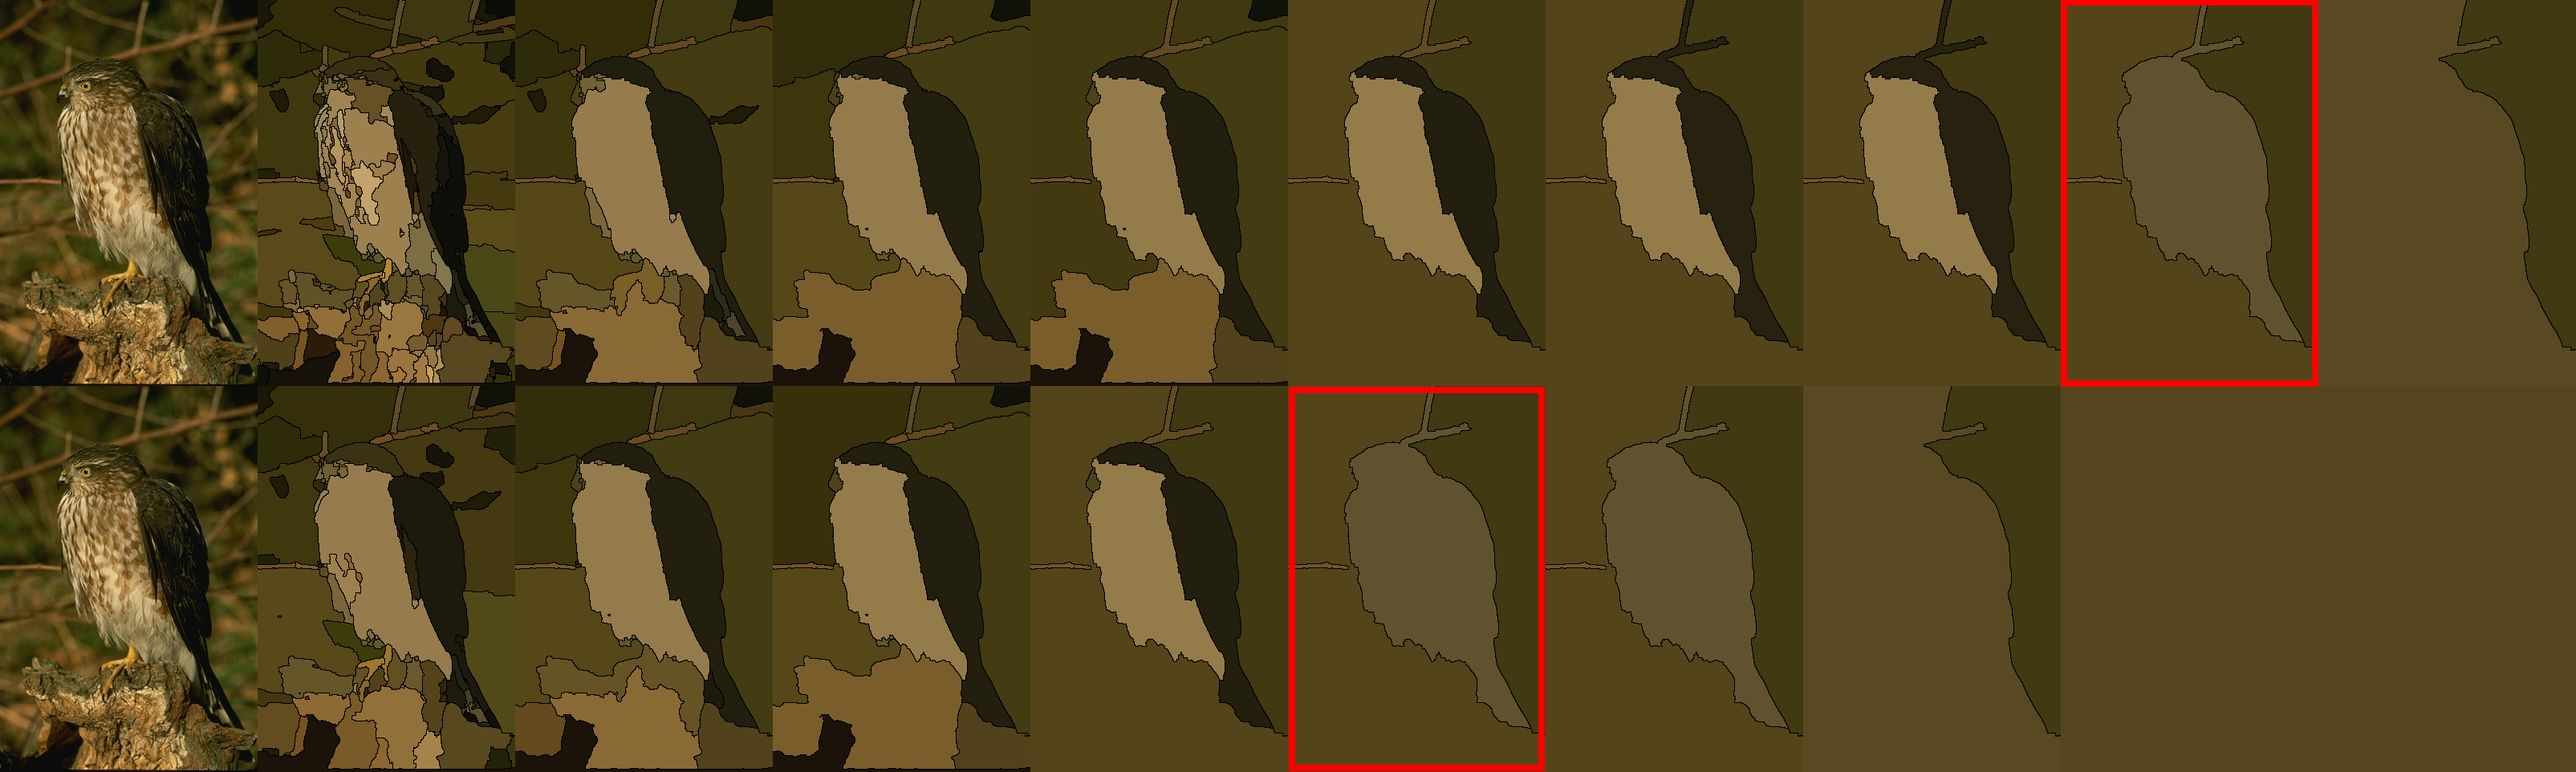
\includegraphics[width=17cm]{fig/vis/70090.png} \\
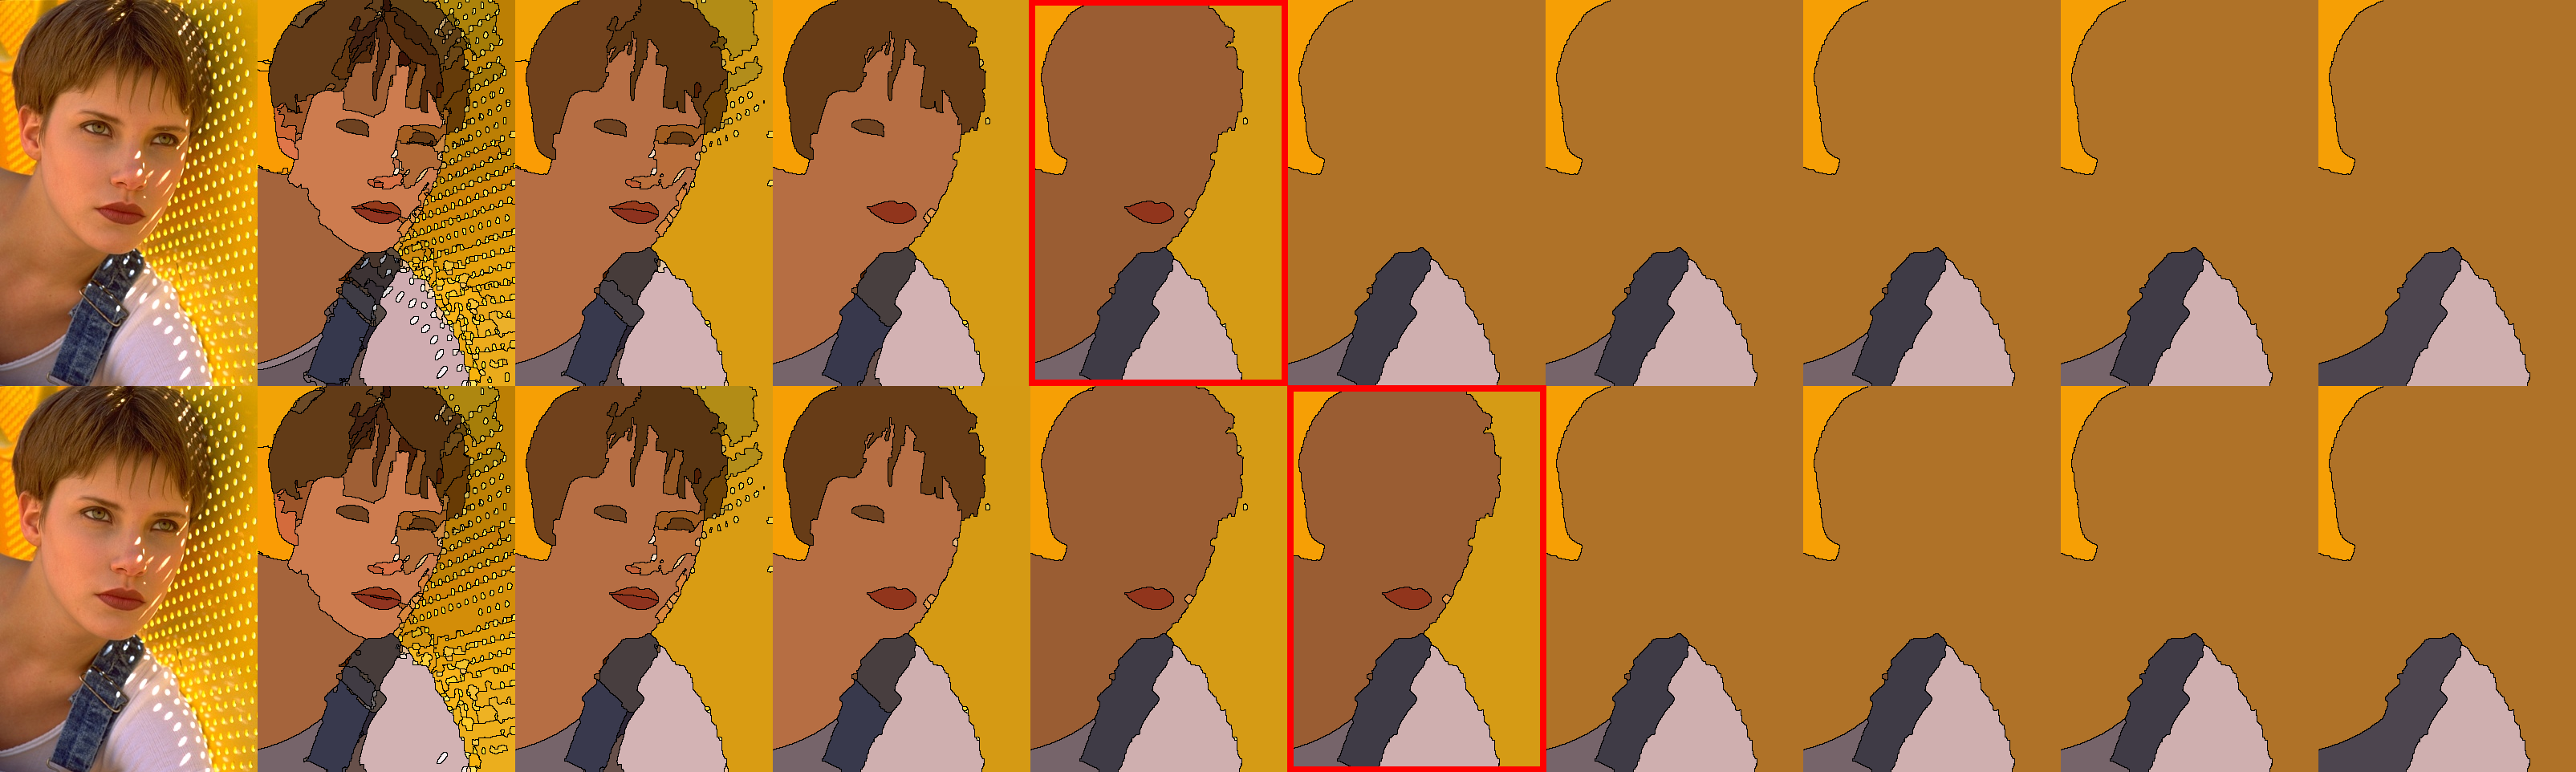
\includegraphics[width=17cm]{fig/vis/388006.png} \\
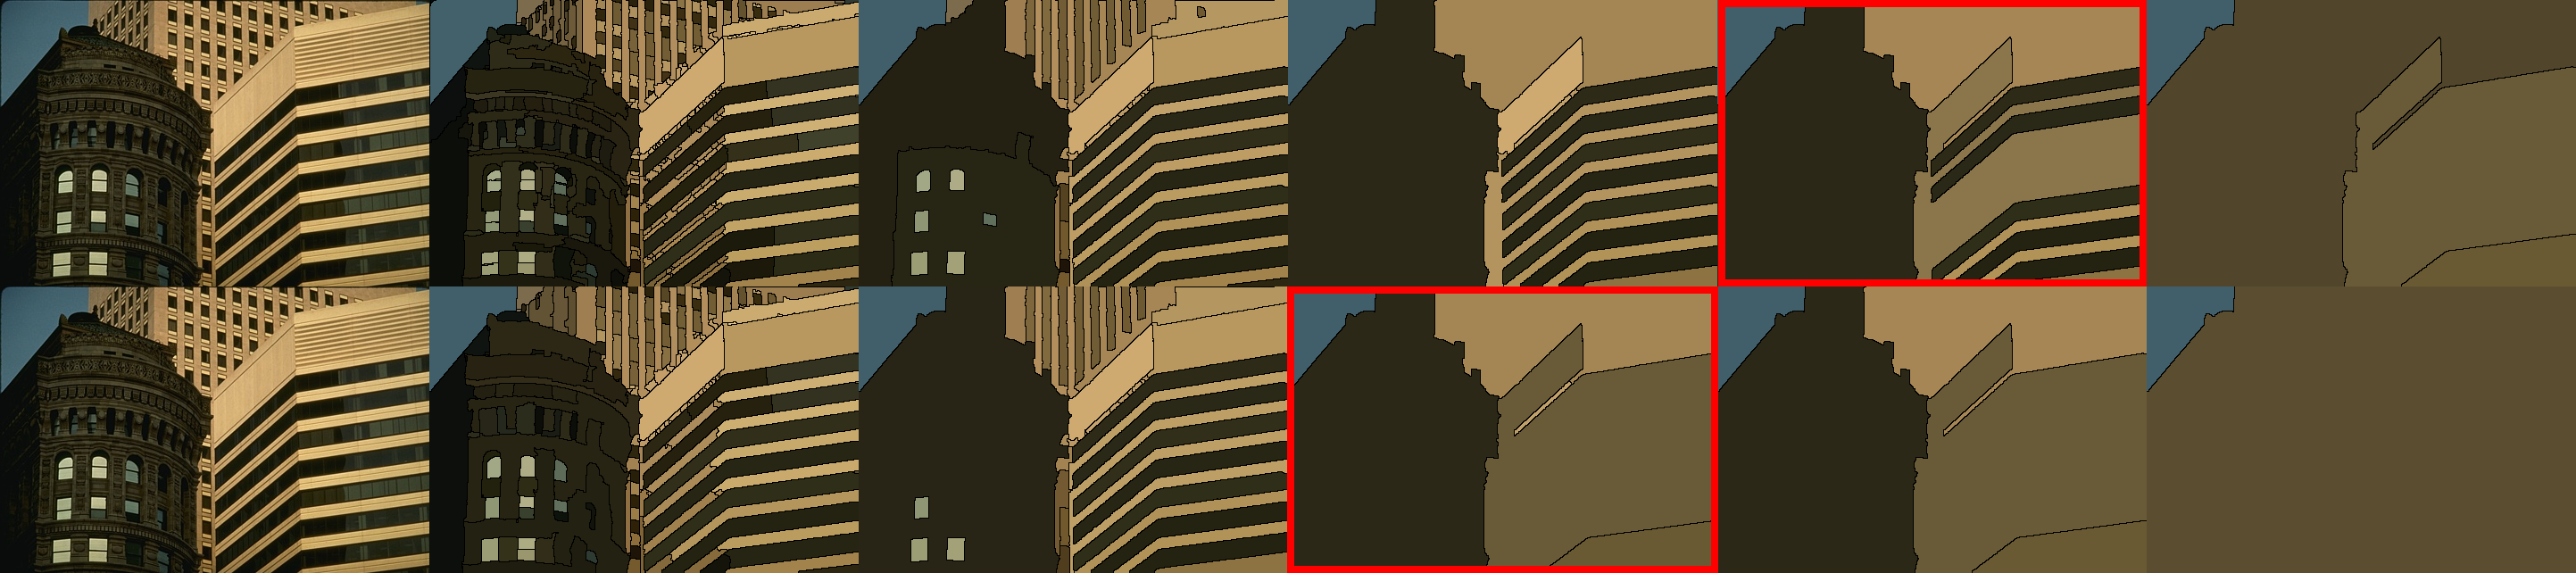
\includegraphics[width=17cm]{fig/vis/48017.png} \\
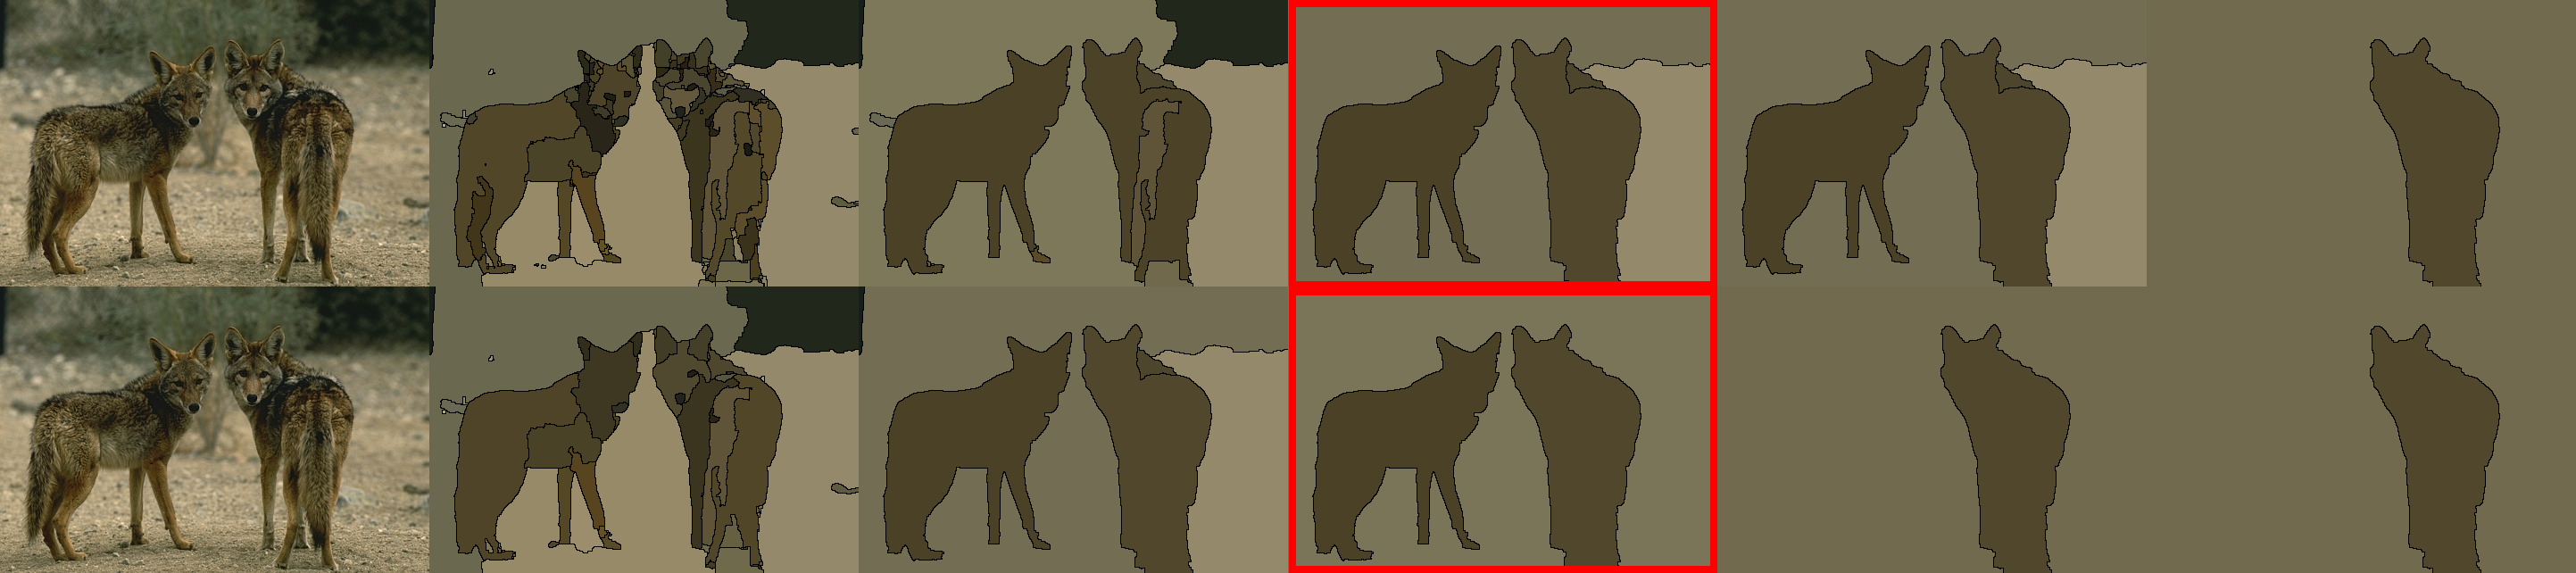
\includegraphics[width=17cm]{fig/vis/196062.png}
\end{tabular}
\end{center}
\caption{Results of MCG(first row) and MCG results improved by our approach(second row). Original images are shown in the left most. Segmentations of optimal-dataset-sclae(ODS) are given in the middle. And from left to right are different scales, from fine to coarse. Red bounding box indicates the scale with best results. It can be seen that our approach provides better alignment, both across images and within one image. }
\label{fig:mcgnimprov}
\end{figure*}
>>>>>>> .r54

<<<<<<< .mine
% % \begin{table}
% \begin{center}
% \resizebox{0.5\textwidth}{!}{
% \begin{tabular} {| c | c | c | c | c | c | c |}
% \hline
% & \multicolumn{2}{|c|}{Covering} & \multicolumn{2}{|c|}{PRI} 
% & \multicolumn{2}{|c|}{VI} \\ \cline{2-7}
%  & ODS & OIS & ODS & OIS & ODS & OIS \\ \hline
% MCG &
% 0.611  & 0.672  & 0.832  & 0.861  & 1.570  & 1.390  \\
% MCG+ours &
% 0.626  & 0.679  & 0.832  & 0.862  & 1.525  & 1.378  \\
% MCG+ global &
% 0.622  & 0.674  & 0.831  & 0.861  & 1.541  & 1.387  \\ 
% \hline
% SCG &
% 0.600  & 0.659  & 0.829  & 0.860  & 1.628  & 1.422  \\ 
% SCG+ours&
% 0.608  & 0.669  & 0.832  & 0.860  & 1.606  & 1.413  \\ 
% SCG+ours(retrained)&
% 0.612  & 0.671  & 0.833  & 0.861  & 1.586  & 1.410  \\ 
% SCG+global&
% 0.612  & 0.667  & 0.830  & 0.860  & 1.582  & 1.415  \\ 
% \hline
% gpb &
% 0.594  & 0.653  & 0.827  & 0.856  & 1.690  & 1.475  \\ 
% gpb+ours&
% 0.603  & 0.660  & 0.828  & 0.857  & 1.659  & 1.465  \\ 
% gpb+ours(retrained)&
% 0.608  & 0.663  & 0.828  & 0.858  & 1.642  & 1.460  \\ 
% gpb+global &
% 0.606  & 0.661  & 0.827  & 0.857  & 1.645  & 1.466  \\ 
% \hline
% PMI &
% 0.533  & 0.585  & 0.760  & 0.813  & 2.025  & 1.822 \\ 
% PMI+ours &
% 0.539  & 0.589  & 0.759  & 0.814  & 2.008  & 1.815 \\ 
% PMI+ours(retrained)&
% 0.543  & 0.590  & 0.760  & 0.815  & 1.996  & 1.813 \\ 
% PMI+global&
% 0.540  & 0.588  & 0.760  & 0.814  & 2.006  & 1.810  \\ 
% \hline
% \end{tabular}}
% \end{center}
% \caption{Benchmark results of other hierarchies. Each segmentation has three entries. The first one shows the original benchmark score of the method. The second entry(+ours) is the score using general regression forest trained by MCG segments. The third entry(+ours retrained) is the results using a regression forest trained by segments from the method itself.}
% \label{tab:res_other_hier}
% \end{table}=======

\begin{figure*}
\begin{center}
\begin{tabular}{l c}
\rotatebox[origin=c]{90}{MCG segmentation} &
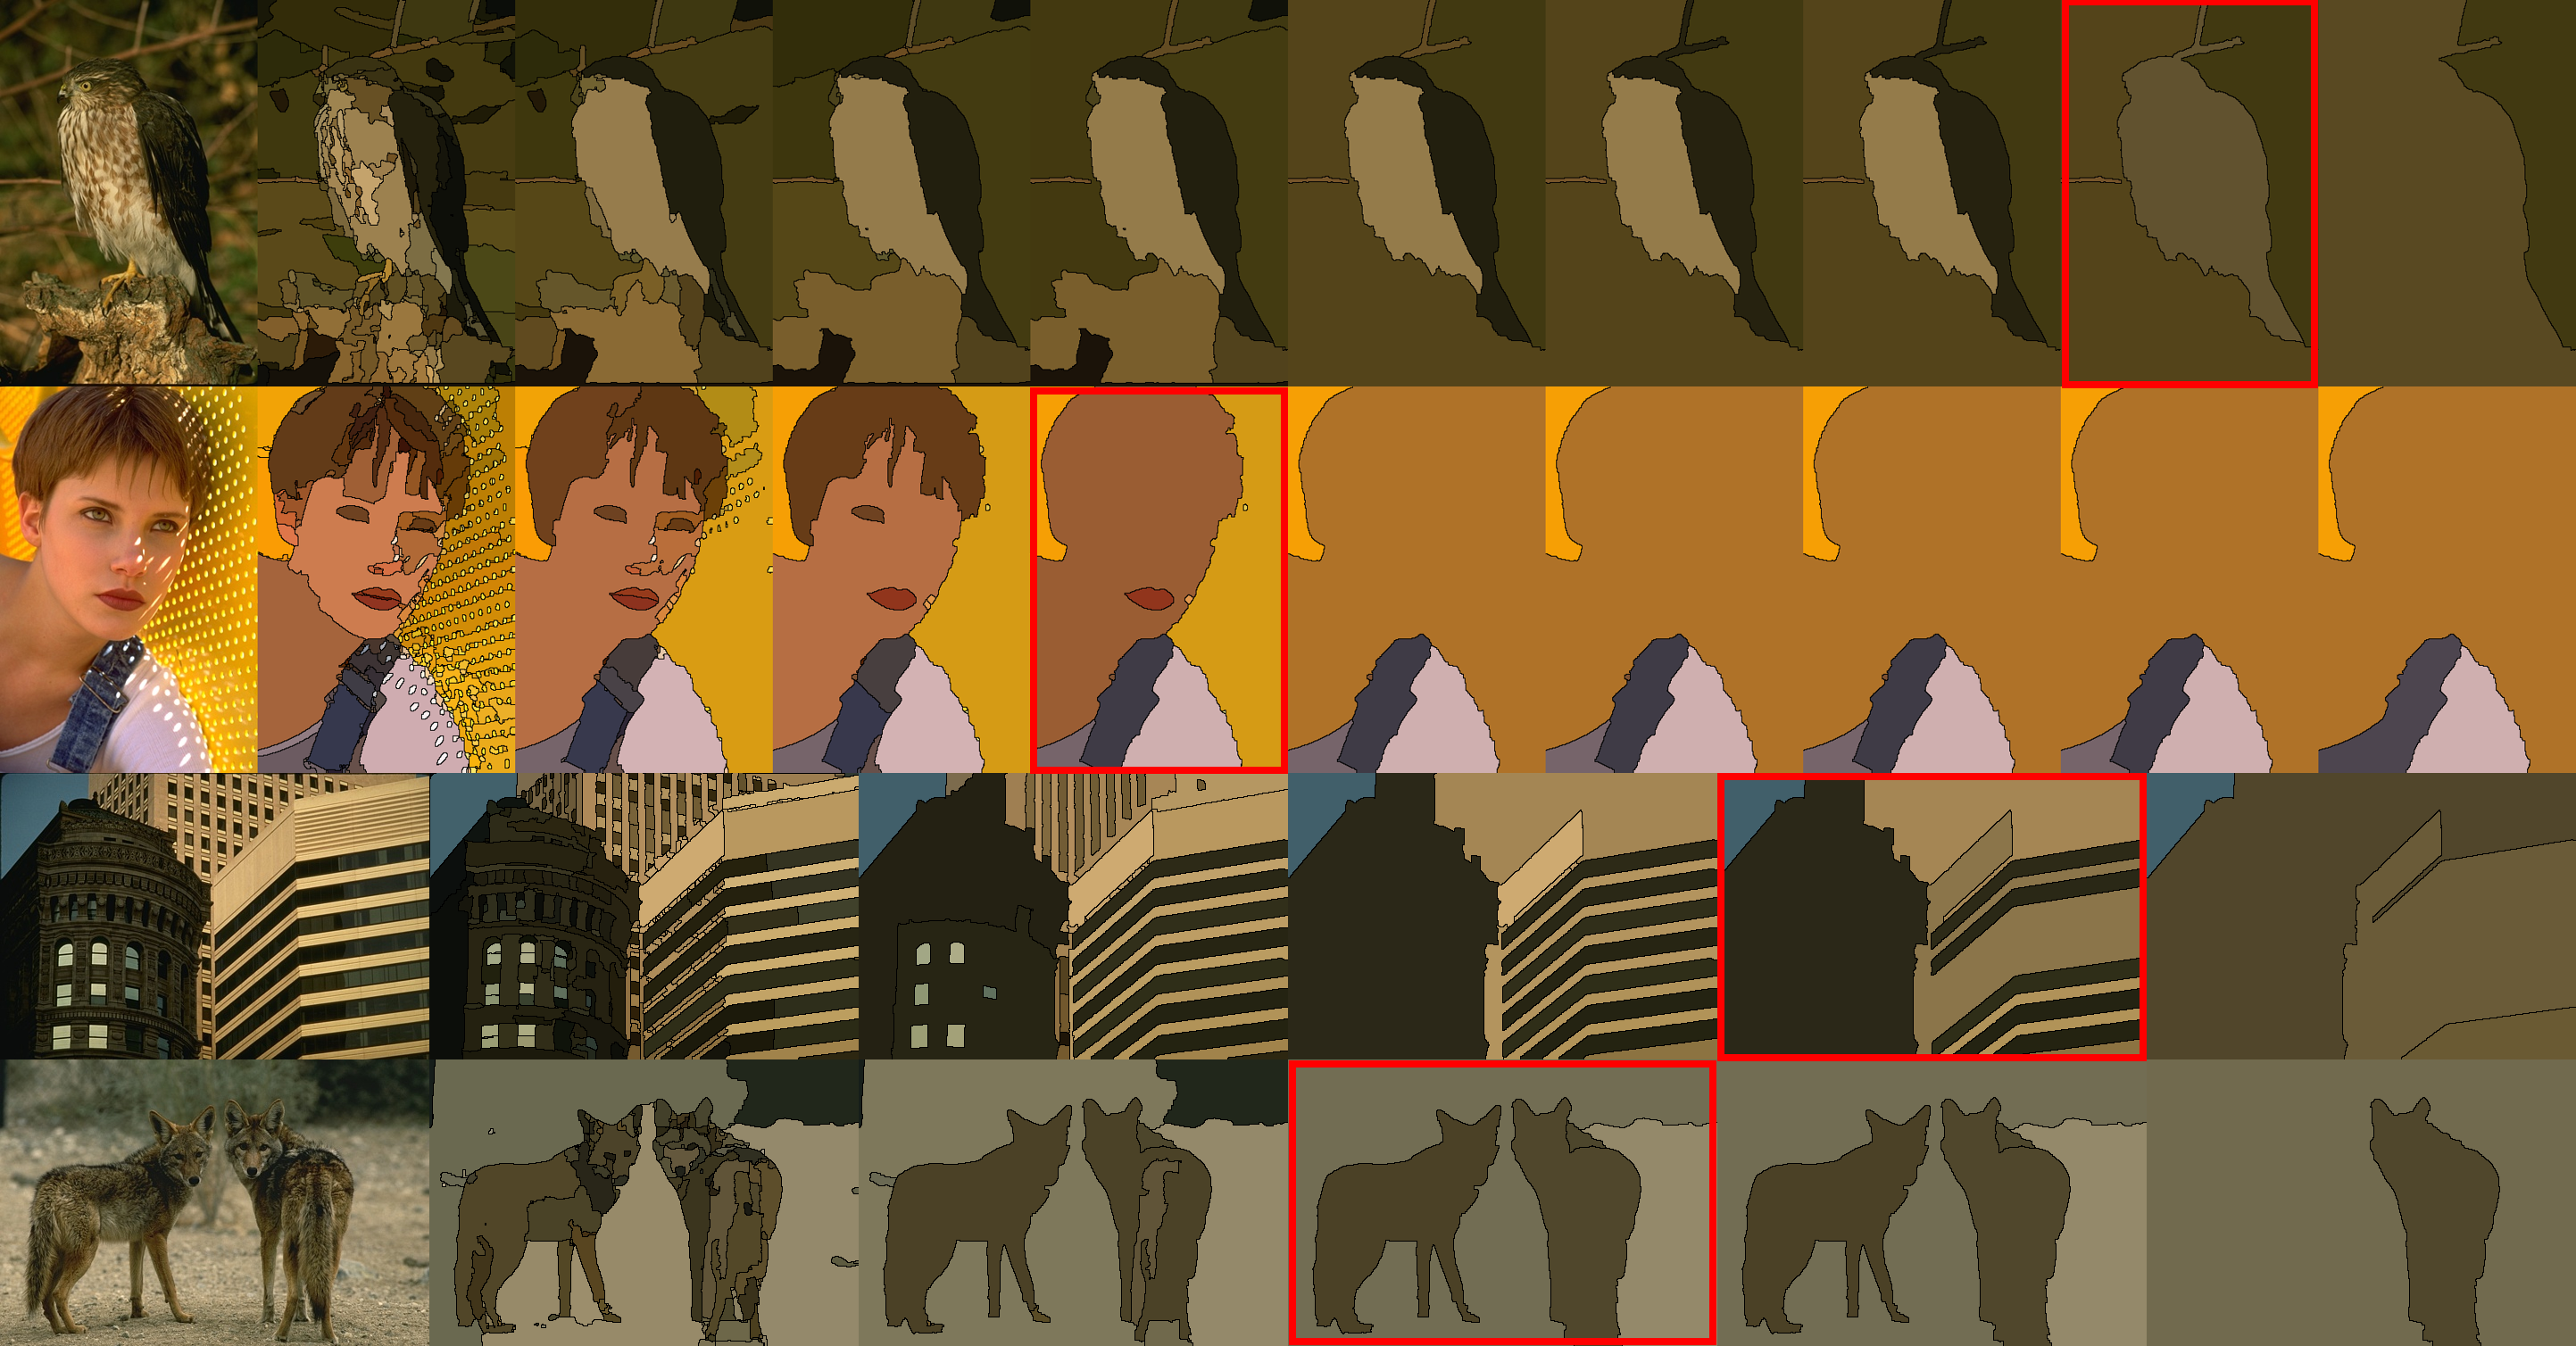
\includegraphics[width=17cm]{fig/vis/stack_1.png} \\
\rotatebox[origin=c]{90}{Our results} &
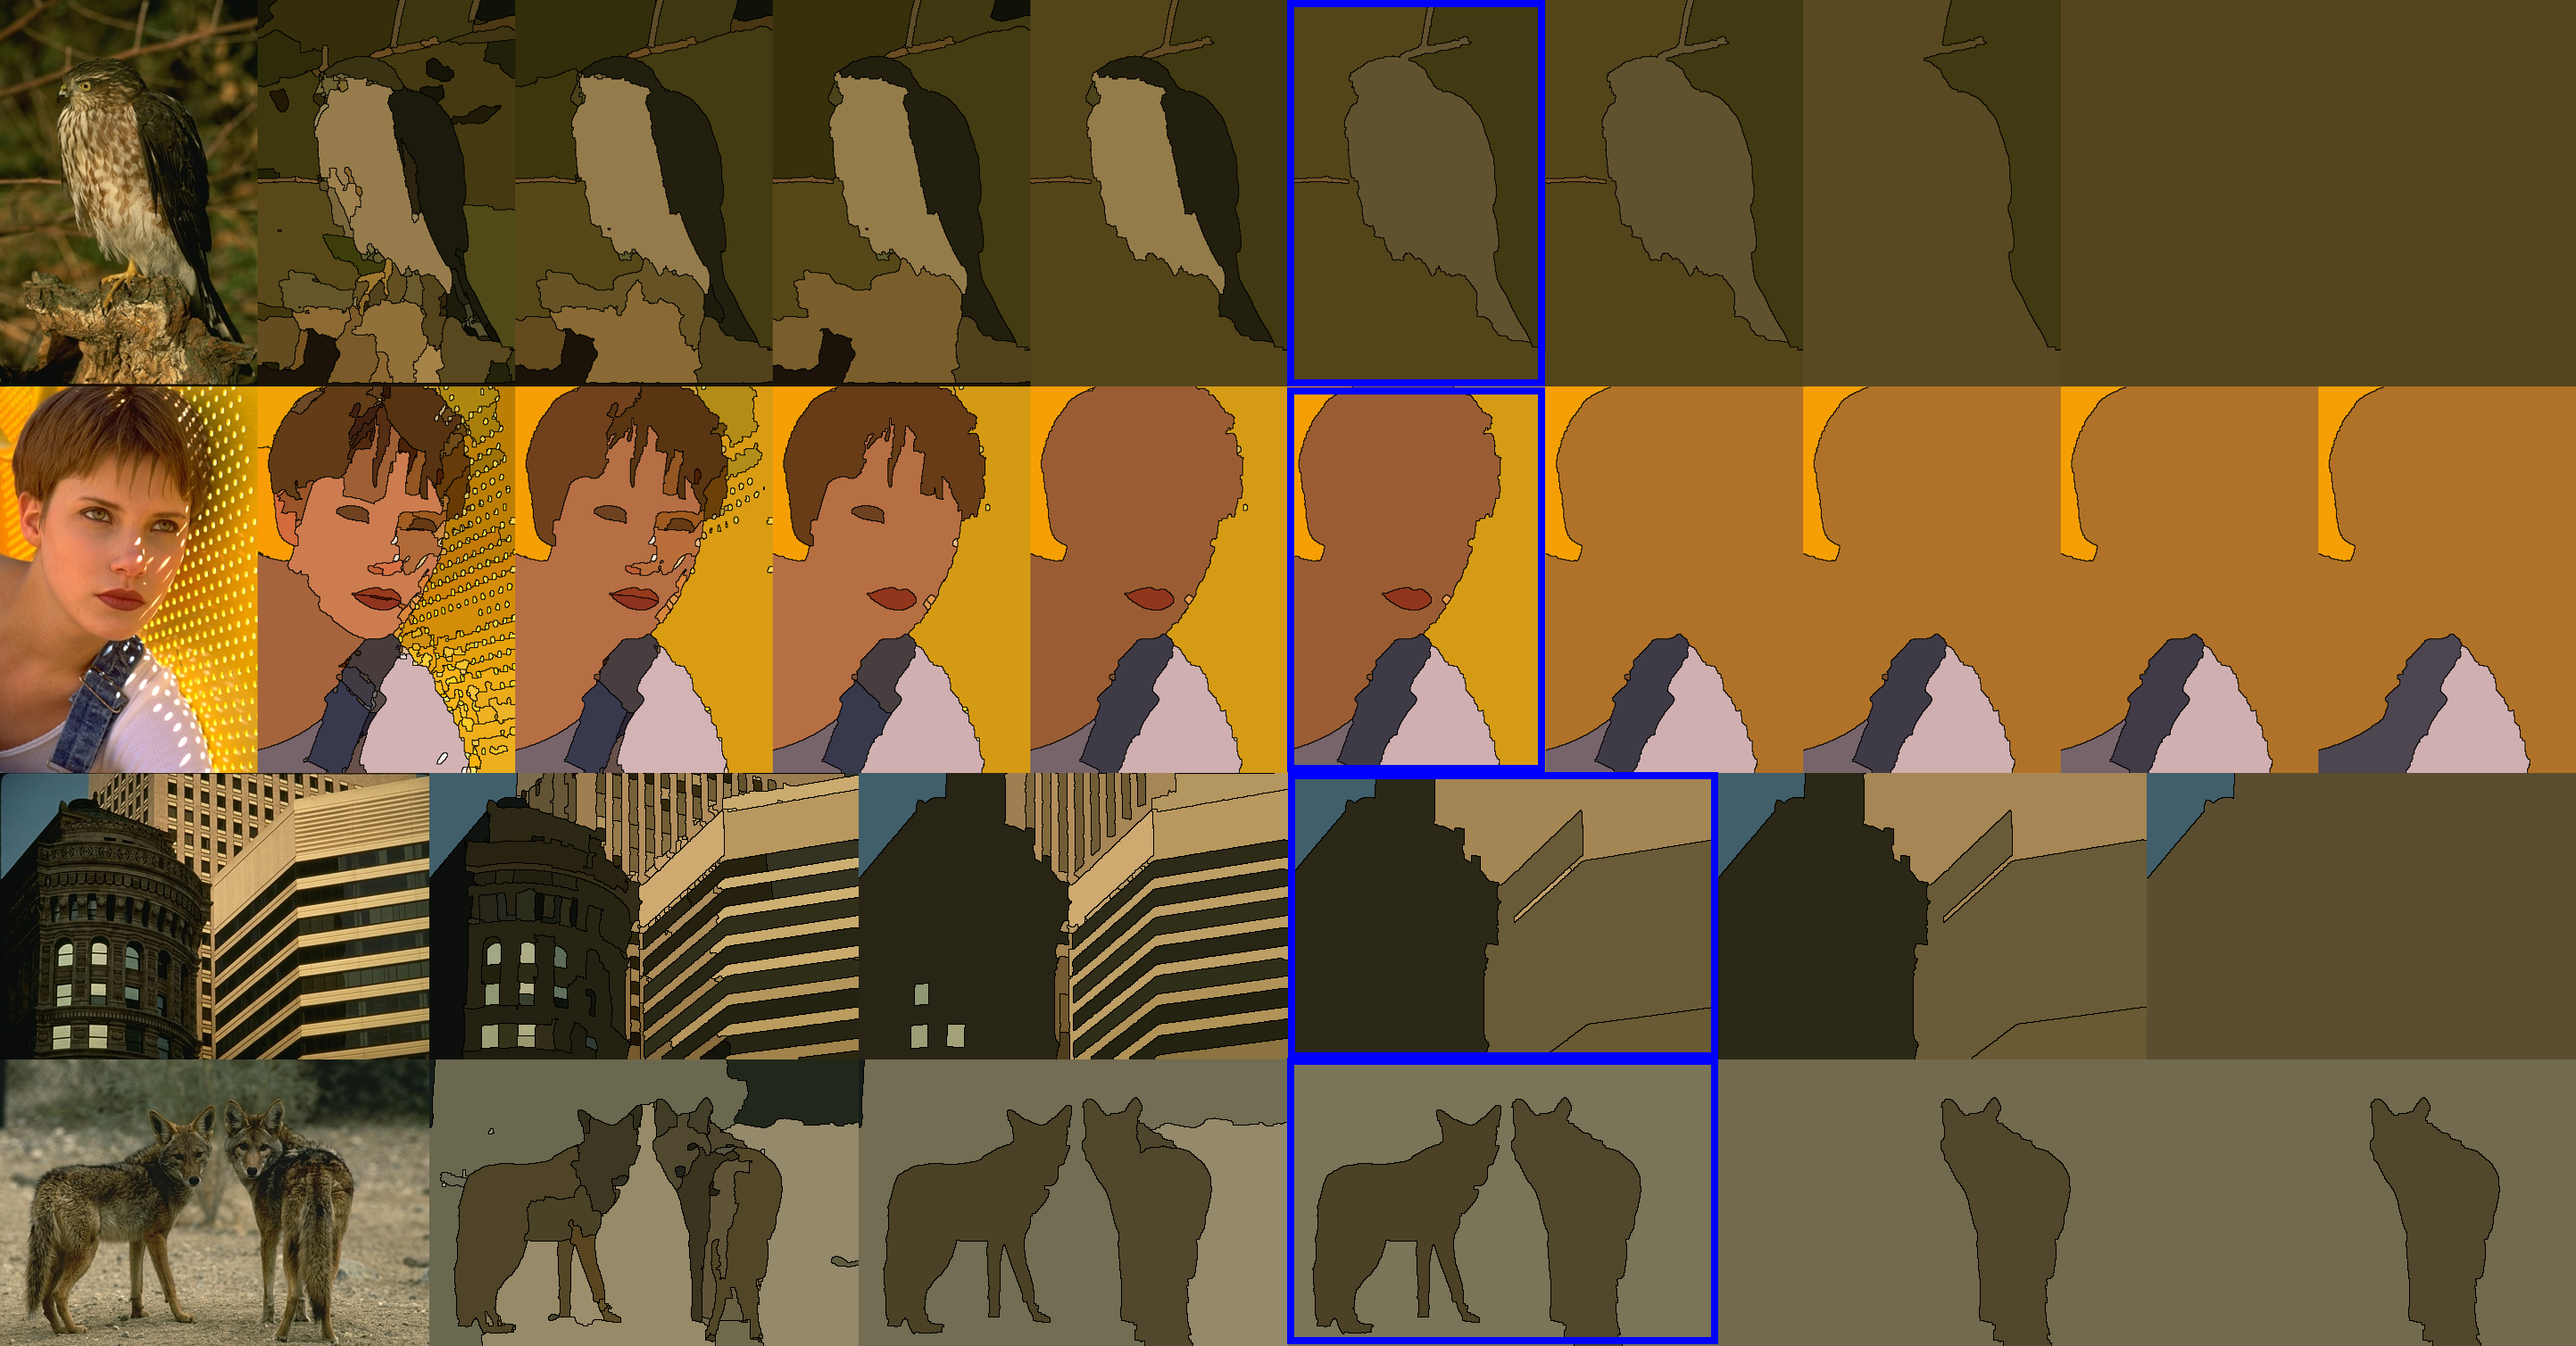
\includegraphics[width=17cm]{fig/vis/stack_2.png} \\
\end{tabular}
\end{center}
\caption{Results of MCG(first row) and MCG results improved by our approach(second row). Original images are shown in the left most. Segmentations of optimal-dataset-sclae(ODS) are given in the middle. And from left to right are different scales, from fine to coarse. Red bounding box indicates the scale with best results. It can be seen that our approach provides better alignment, both across images and within one image. }
\label{fig:mcgnimprov2}
\end{figure*}>>>>>>> .r54
